\chapter{Kvalitetskontroll og forbedring}
\label{kap:kvalitetskontroll} % Opprinnelig kapittelnr: 15

\section{Innledning}
Statistiske metoder har anvendelsesmuligheter ved  kvalitetskontroll av
mas\-se\-produserte artikler og overvåking av prosessser.
Vi kan f.eks. være inte\-ressert i å
estimere andelen defekte artikler i et større produksjonsparti på
grunnlag av et utvalg av artikler (hypergeometrisk situasjon), eller estimere
defektsannsynligheten i en løpende produksjonsprosess (binomisk situasjon),
eller kvaliteten av artiklene i en løpende produksjon 
(måle\-situa\-sjon). Slike problemer kan angripes ved de metodene som er
utviklet i Kapittel 7 og 8.

Hensikten med  kvalitetskontroll kan være å avgjøre om et
gitt produksjonsparti ikke lever opp til en ønsket kvalitet,
eller å avgjøre om en produksjonsprosess er ute av kontroll,
dvs. sjekke om defektsannsynligheten i produksjonen viser økende
tendens, eller sjekke om prosessen gir dårligere målt
kvalitet enn før.  Slike situasjoner kan ofte betraktes som et 
beslutningsproblem under usikkerhet med to mulige beslutninger.  I tilfellet
med produksjonspartiet, akseptere det og sende partiet til kunden eller
forkaste partiet. I tilfellet med produksjonsprosessen, la den fortsette eller
stoppe den for justering.  

Vi finner analoge problemstillinger innen revisjon, når generelle
konklusjoner trekkes på grunnlag av stikkprøver. Det kan dreie seg
om konklusjoner mht. feilhyppighet og beløpsmessig feil i en gitt
populasjon av objekter (f.eks. bilag), eller tilsvarende for en administrativ
 prosess.

Dette kan formuleres som hypotesetestingsproblemer, men det er ofte
 hensiktsmessig med terminologi tilpasset anvendelsesområdet.
I dette kapitlet er kvalitet  i produksjonssituasjoner i fokus.
For bruk av tilsvarende metoder i revisjon, se Lillestøl (1996).

I de senere år har interessen innen kvalitetsarbeid gått mer over mot
metoder for forbedring av prosesser, dvs. reduksjon av
defekt/feil\-sann\-syn\-lig\-heter  og økning av forventet målt kvalitet
og/eller reduksjon i variasjon i kvalitet. Vi gir en kort omtale av slike 
problemstillinger i et avsluttende avsnitt.

Dette kapitlet vektlegger koblingen mellom kvalitetskontroll/forbedring og
sannsynlighetsteori/statistisk teori. For nærmere beskrivelse av hvordan
id\'{e}ene tillempes i praksis må vi vise til spesiallitteratur.



\section{Kontroll av produksjonsparti}
Vi antar at en artikkel masseproduseres.  Hver artikkel kan klassifiseres som
enten defekt eller intakt.  Man vil selvsagt helst levere bare intakte 
artikler, men en undersøkelse av alle artiklene før de leveres er ofte
ikke hensiktsmessig.  Det kan enten være for tidkrevende og/eller dyrt
eller det kan skade artiklene, kanskje også ødelegge dem (f.eks.
dersom artiklene er fyrverkerisaker).  Anta at artiklene produseres i partier
på et gitt antall enheter.  Av de grunner som er nevnt velger vi å
trekke ut et visst antall enheter tilfeldig fra hvert parti og undersøke
disse, telle opp antall defekte og akseptere resten av partiet dersom antall 
defekte i utvalget er lite.  La oss innføre følgende notasjon 
vedrørende kvalitetskontroll av et gitt parti.
\begin{center}
\begin{tabular}{ccl}
   $N$ & = & antall partikler i partiet\\
   $n$ & = & antall artikler i utvalget \\
   $M$ & = & antall defekte artikler i partiet \\
   $Y$ & = & antall defekte artikler i utvalget \\
   $k$ & = & aksepttall \\
$\theta $& = &$M/N$ brøkdelen av defekte i partiet
\end{tabular}
\end{center}
\noindent Vår kontrollplan innebærer altså at partiet aksepteres
dersom $Y\leq k$, forkastes dersom $Y>k$, hvor $k$ er en konstant som velges slik
at planen får ønskede egenskaper.  Vi ønsker selvsagt ikke at 
et parti med få defekte skal bli forkastet, på den annen side 
ønsker vi heller ikke at et parti med mange defekte skal bli akseptert.
Dette er motstridende krav som spiller inn når $k$ skal velges fornuftig.
Hvordan en gitt plan virker i ulike situasjoner kan studeres ved å 
beregne sannsynligheten for å akseptere partiet som funksjon av $\theta$:

\begin{eqnarray*}
K(\theta )&=&P_{\theta}(\mbox{Akseptert parti}) \\
          &=&P_{\theta}(Y\leq k)=\sum_{y=0}^k P_{\theta}(Y=y)
\end{eqnarray*}
\noindent hvor $P_{\theta}$ betegner sannsynlighet beregnet under forutsetning
av at brøkdelen defekte i hele partiet er $\theta$. Funksjonen $K(\theta )$
vil vi kalle {\em karakteristikken} til den gitte plan.  Den vil her være
en avtagende funksjon av $\theta$.  Valget av $n$ og $k$ vil være 
bestemmende for karakteristikken.  For gitt $n$ vil, uansett $\theta, 
K(\theta )$ øke med $k$, dvs. sjansen for både ønsket og uønsket
aksept øker med $k$, og konsekvensene av dette må vurderes ved valg av
$k$ og $n$.

Siden utvalget på $n$ skjer tilfeldig (uten tilbakelegging), er vi i en 
hypergeometrisk situasjon, dvs. $Y$ er hypergeometrisk fordelt ($N, N\theta ,
n$).  Følgelig er

\[  P_{\theta}(Y=y)=\frac{\bino{N\theta }{y} \cdot 
         \bino{N(1-\theta )}{n-y}}{\bino{N}{n}} \]

\noindent og slike sannsynligheter kan, for ulike $\theta$ , i prinsippet beregnes
direkte eller ved bruk av tabeller.  Dette er imidlertid ofte brysomt.
I mange situasjoner er partistørrelsen $N$ stor og utvalgsstørrelsen
$n$ forholdsvis liten.  Vi har sett i Kapittel 6.3 at vi da kan bruke
binomiske sannsynligheter som tilnærmelse til hypergeometriske
sannsynligheter (repeter hvorfor!), dvs.

\[  P_{\theta}(Y=y) \approx \bino{n}{y}{\theta}^y{(1-\theta )}^{n-y} \]

\noindent Dersom $\theta$ er liten og $n$ er stor, men fremdeles liten i forhold
til $N$, vet vi at binomiske sannsynlighet kan tilnærmes med
Poissonsannsynligheter (Se Kapittel 6.4), slik at 

\[  P_{\theta }(Y=y) \approx \frac{{(n\theta )}^y}{y!}e^{-n\theta} \]
Det er grunn til å merke seg at så lenge populasjonen $N$ er 
stor i forhold til utvalget $n$, vil den eksakte populasjonsstørrelse
ikke spille noen rolle, den forsvinner i den binomiske (og Poisson) 
tilnærmingen.  Eksempelvis får vi en situasjon med $n = 10$, 
tilnærmet samme karakteristikk for $N = 1000$ som for $N = 10000$.
I noen situasjoner kan det også komme på tale å bruke 
normaltilnærmelse til de hypergeometriske (binomiske) 
sannsynlighetene. \\

\begin{eksempel}{Kontrollplan-karakteristikk}
I en situasjon hvor $N$ = 8 og vi har valgt $n$ = 4 og $k$ = 1 blir
$\theta = M/8$, og karakteristikken blir da
\begin{eqnarray*}
K(\theta )&=&\sum_{y=0}^1 P_{\theta }(Y=y) \\
          &=&\frac{\bino{M}{0}\cdot \bino{8-M}{4}}{\bino{8}{4}}+
             \frac{\bino{M}{1}\cdot \bino{8-M}{3}}{\bino{8}{4}}
\end{eqnarray*}

\noindent Funksjonen er definert for $M$ = 0, 1, 2, \ldots, 8, og verdiene er
 gitt ved (sjekk!)

\begin{center}
\begin{tabular}{l|ccccccccc}
 $M$         & 0 & 1 & 2 & 3 & 4 & 5 & 6 & 7 & 8\\ \hline
$K(\theta )$ & 1 & 1 &$\frac{55}{70}$&$\frac{35}{70}$&$\frac{17}{70}$&
                       $\frac{5}{70}$& 0 & 0 & 0
\end{tabular}
\end{center}

\noindent Leseren kan selv sammenligne denne plan med alternative planer, se
Oppgave~1.\\
\end{eksempel}

\begin{eksempel}{Kontrollplan-karakteristikk}
Et mer realistisk eksempel har vi når $N$ = 1000 og $n$ = 50.  Anta 
at vi velger en plan med $k$ = 2.  I dette tilfellet er binomisk 
tilnærmelse ganske god, og Poisson tilnærmelse brukbar for liten
$\theta = M/N$.  Vi har følgende karakteristikk


\begin{eqnarray*}
K(\theta )&=&\sum_{y=0}^2 \frac{\bino{N\theta }{y} \cdot 
         \bino{N(1-\theta )}{50-y}}{\bino{1000}{50}}
 \\
     &\approx&\sum_{y=0}^2 \bino{50}{y}{\theta}^y{(1-\theta )}^{50-y} 
     \approx  \sum_{y=0}^2 \frac{{(50\theta )}^y}{y!}e^{-50\theta}
\end{eqnarray*}

\noindent Det siste uttrykket er inntegnet i Figur~\ref{fig:karakteristikk} som om $\theta $ varierer
kontinuerlig i intervallet fra 0 til 1.  Vi ser at et parti med 5 \%
defekte har ca. 54 \% sjanse for å bli akseptert, mens et parti med
10 \% defekte har ca. 12 \% sjanse for å bli akseptert.  Leseren 
kan selv sammenligne denne plan med alternative planer.
\end{eksempel}

\begin{figure}[ht]
\centering
	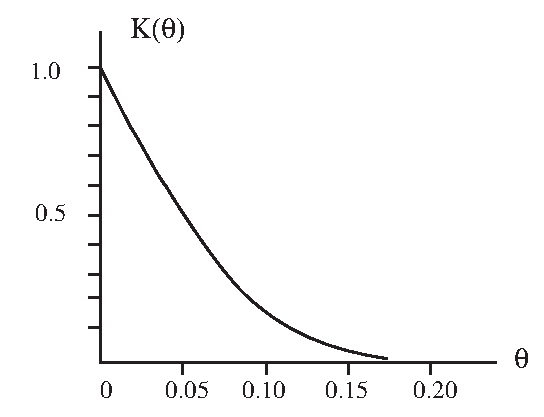
\includegraphics[scale=1.0]{figurer/fig15_1.pdf} 
\caption{Karakteristikk}
	\label{fig:karakteristikk}
\end{figure}

Det kan være aktuelt å spesifisere andeler
 ${\theta}_1$ og ${\theta}_2$ (${\theta}_1<{\theta}_2$), slik at aksept er
ønskelig hvis $\theta \leq {\theta}_1$ mens forkasting er
ønskelig hvis $\theta \geq {\theta}_2$.  I denne forbindelse taler
man ofte om 
\begin{eqnarray*}
\mbox{Produsentens risiko}&=&\max_{\theta \leq \theta_1}(1-K(\theta ))
                                                   = (1-K(\theta_1)) \\
\mbox{Konsumentens risiko}&=&\max_{\theta \geq \theta_2}K(\theta ) = K(\theta_2) 
\end{eqnarray*}
\noindent men disse begreper er ikke entydige, idet valget av ${\theta}_1$ og
${\theta}_2$ vil være delvis vilkårlig.  Illustrer produsentens
og konsumentens risiko i Figur~\ref{fig:karakteristikk}!

En kontrollplan er ikke fullstendig spesifisert med mindre man også
angir hva som skal foretas med aksepterte og forkastede partier.  Her
foreligger mange muligheter, og hva som gjøres vil i praksis avhenge
av omstendighetene.
Et akseptert parti kan f.eks. videresendes med eventuelle defekte som er
funnet, eventuelt til redusert pris.  De funne defekte kan være
fjernet, eller de kan være erstattet med nye artikler som er 
kontrollert, evt. ikke kontrollert.  Et forkastet parti kan vrakes i 
sin helhet, dette vil f.eks. alltid være tilfellet dersom artiklene
ødelegges i kontrollen.  Alternativt kan man, dersom det er økonomisk
forsvarlig, foreta en fullstendig kontroll av det forkastede parti med
sikte på å erstatte alle defekte artikler med intakte.

Et aktuelt begrep i forbindelse med vurdering av egenskapene til en
fullstendig spesifisert kontrollplan er {\em forventet utgående
kvalitet} $Q(\theta )$ som gir uttrykk for forventet andel defekte i
leverte partier som funksjon av andel defekte i partiet før kontrollen.
Begrepet er først og fremst aktuelt å bruke i situasjoner der artikler
ikke ødelegges i kontrollen og defekte artikler kan erstattes.

Den enkleste situasjon har vi dersom et akseptert parti videresendes 
med de defekte som er funnet, mens et forkastet parti blir underlagt
fullstendig kontroll der alle defekte erstattes med intakte.  Forventet
utgående kvalitet er da

\[  Q(\theta )=Q_1(\theta )=\theta K(\theta ) \]

\noindent idet sannsynligheten for å akseptere et parti med en andel
$\theta$ defekte er $K (\theta)$, mens for et forkastet parti er antall leverte
defekte null, og det skjer med sannsynlighet $1 - K (\theta)$.

En mer realistisk situasjon vil være at også de funne defekte
i aksepterte partier erstattes med intakte.  Forventet utgående 
kvalitet blir da isteden

\[  Q(\theta )=Q_2(\theta )=\sum_{y=0}^k \frac{M-y}{N}P_{\theta}(Y=y) \]

\noindent idet, dersom vi finner $y$ defekte og aksepterer resten av partiet 
$(y\leq k)$, er det $M-y$ gjenværende defekte blant de $N$ 
artiklene, mens dersom partiet forkastes $(y>k)$, vil det leverte parti
overhodet ikke inneholde defekte.

For planer av den typen vi har betraktet her, vil $Q(\theta)$ være
liten når $\theta$ er liten, siden partiet da allerede er godt 
før kontrollen.  Den er liten også når $\theta$ er stor
siden vi da har stor sjanse for å forkaste partiet, foreta en 
fullstendig kontroll og levere feilfritt parti.  Mellom disse to
ytterlighetene vil typisk funksjonen $Q(\theta)$ ha et maksimum
${\theta}_0$.  Er dette maksimum lite vil kvaliteten av leverte partier
være god uansett hvor mange defekte det opp\-rin\-ne\-lig var i partiet.
Den første av de to planene ovenfor er spesielt enkel å analysere
da forventet utgående kvalitet kan beregnes ut fra karakteristikken
alene.  For store $N$, slik tilfellet ofte er i praksis, vil de to 
formlene ovenfor tilnærmet gi samme svar. \\

\begin{eksempel}{Utgående kvalitet}
For kontrollplanen i Eksempel 1 der $N$ = 8, og $n$ = 4 og $k$ = 1 blir
forventet utgående kvalitet for de to framgangsmåtene beskrevet 
ovenfor henholdsvis (sjekk tallene!)
\begin{center}
\begin{tabular}{|c|ccccccccc|} \hline
$M$ &   0   &   1   &   2   &   3   &   4   &   5   &  6   &  7  &  8\\ \hline
$Q_1(\theta )$& 0 & 0.125 & 0.196 & 0.188 & 0.121 & 0.045 &  0  &  0  &  0 \\
$Q_2(\theta )$& 0 & 0.063 & 0.125 & 0.134 & 0.093 & 0.036 & 0 & 0 & 0\\ \hline
\end{tabular}
\end{center}
Vi ser at forventet defektprosent til forbruker som ventet alltid er
lavere ved den siste framgangsmåten enn den første.  Videre ser vi
at maksimal forventet defektprosent er henholdsvis 19.6 \% og 13.4 \%.
Dette inntreffer dersom antall defekte $M$ i partiet er henholdsvis 
2 og 3 (25 \% og 37.5 \%).  I praksis vil selvsagt $M$ variere fra parti
til parti, med de nevnte verdier vil altså være de minst gunstige
for forbrukeren.
\end{eksempel}


\begin{eksempel}{Utgående kvalitet}
For kontrollplanen i Eksempel 2, der $N$ = 1000, $n$ = 50 og $k$ = 2,
 får vi 
\begin{center}
\begin{tabular}{|c|cccccc|} \hline
$\theta$     &   0.01  &  0.02  &  0.04  &  0.05  &  0.06  &  0.10  \\ \hline
$K(\theta )$        & 0.986 & 0.920 & 0.677 & 0.544 & 0.423 & 0.125 \\
$\theta K(\theta )$& 0.009 & 0.018 & 0.027 & 0.027 & 0.025 & 0.012 \\ \hline
\end{tabular}
\end{center}
Siste linje i denne tabellen er altså forventet utgående kvalitet
$Q_1(\theta)$ for den første framgangsmåten.  Beregnes 
$Q_2(\theta)$ vil denne avvike fra $Q_1(\theta)$ med høyst en enhet
i siste desimal.  Vi ser at partier med lav defektprosent (opp til 2 \%)
gir ubetydelig lavere defektprosent til forbruker, mens for defektprosent 
omkring 5 \%, er defektprosenten til forbruker halvert, mens for partier
med defektprosent på 10 \% vil defektprosenten til forbruker igjen
være av størrelsesorden 1 \%.  Vi ser at den maksimale forventede
defektprosent til forbruker er ca. 2.7 \%, som inntreffer for partier
hvor defektprosenten er 4 - 5 \%.
\end{eksempel}

Den utvalgsplanen som er beskrevet ovenfor er spesielt enkel.  Det 
finnes andre og mer kompliserte planer som kan være aktuelle i visse
situasjoner.  Mest aktuelt er kanskje utvalgsplaner i to trinn:  Først
trekkes et utvalg, og dersom antall defekte er spesielt lite aksepteres
partiet. Dersom antall defekte er spesielt stort forkastes partiet,
mens dersom antall defekte er moderat trekkes et nytt utvalg hvoretter
beslutningen om aksept eller forkastning foretas.  Fordelen ved trinnvise
planer er at de kan redusere omkostningene til kontroll, f.eks. ved at
et dårlig parti avsløres etter kontroll av et lite antall artikler.


\section{Prosesskontroll}
Anta at vi har en produksjonsprosess som, når den er i kontroll, gir
artikler med kvalitet som har en forventning ${\mu}_0$ og standardavvik
$\sigma$.  Både ${\mu}_0$ og $\sigma$ antas kjent, de er anslått 
på grunnlag av et stort antall artikler i en prøveproduksjon.
Når den ordinære produksjon settes i gang ønsker man å
holde kvaliteten under oppsikt ved at man ved regelmessige intervaller
(f.eks. hver time) kontrollerer et visst antall artikler $n$.
Gjennomsnitts-kvaliteten av disse $\bar{X}$ noteres.  Det er 
hensiktsmessig å plotte de gjennomsnittene som er beregnet ved 
suksessive tidspunkter i et {\em kontrolldiagram}.

Dersom forutsetningen i målemodellen er oppfylt, og prosessen 
fortsatt i kontroll, vil $\bar{X}$ ha forventning ${\mu}_0$ og 
standardavvik $\sigma /\sqrt{n}$.  Vi kan derfor alternativt plotte den 
standardiserte størrelse

\[    Z=\frac{\bar{X}-{\mu}_0}{\sigma /\sqrt{n}} \]

\noindent Dette er gjort i Figur~\ref{fig:kontrolldiagram}, kalt $\bar{X}$-diagram.
Betraktningene gjelder også for tilfellet $n=1$, og da har vi et
kontrolldiagram for individuelle observasjoner, et $X$-diagram.

\begin{figure}[ht]
\centering
 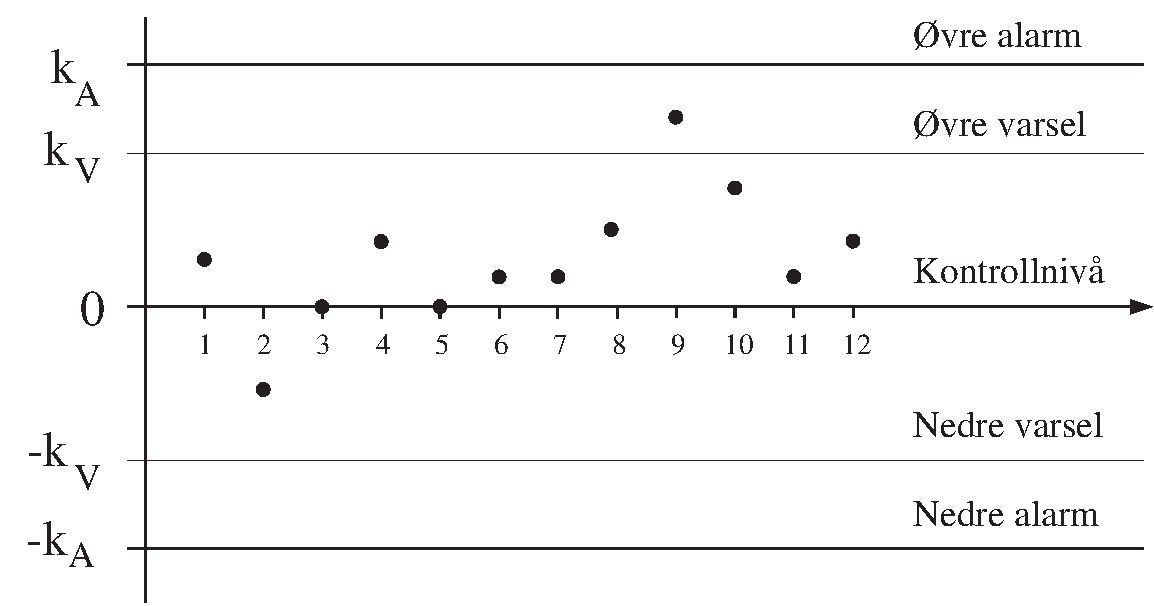
\includegraphics[scale=0.6]{figurer/fig15_2.pdf} 
\caption{Kontrolldiagram}
	\label{fig:kontrolldiagram}
\end{figure}

\noindent Så lenge prosessen er i kontroll, vil $Z$'ene variere omkring 
nullnivå, ekstreme observasjoner kan tyde på at noe er skjedd.  
I figuren er lagt inn to såkalte alarmgrenser, straks et gjennomsnitt
faller utenfor en av disse tolkes det som om prosessen en ute av kontroll,
og nærmere gransking av årsaken settes i gang, eventuelt stoppes
den løpende produksjon.

Vi antar at problemets natur er slik at kvaliteten bør ligge på 
nivået ${\mu}_0$, økning eller senkning av dette er lite ønskelig
eller like interessant, følgelig har vi to alarmgrenser, en på
hver side.

En alarm kan være falsk i den forstand at prosessen fremdeles er i
kontroll, men et gjennomsnitt falt tilfeldigvis utenfor.  Problemet er
derfor å legge alarmgrensene slik at man på den ene side unngår
falske alarmer i rimelig grad, men på den annen side har rimelig 
sjanse til å oppdage relativt raskt en eventuell betydningsfull
endring av kvalitetsnivået.  Man finner det ofte hensiktsmessig også
å legge inn to varselgrenser i figuren, en på hver side av 
kontrollnivået.  Disse brukes gjerne slik at dersom to eller flere
etterfølgende punkter faller mellom varselgrensen og den tilhørende
alarmgrensen så gir dette indikasjon på at prosessen kan være
ute av kontroll.  Hovedspørsmålet er nå hvor alarmgrensen og 
eventuelt varselgrensene bør legges for at de målsettinger som er
uttrykt ovenfor blir oppfylt.

Dersom produksjonsprosessen er i kontroll, slik at forutsetningen i 
måle\-modellen om uavhengighet for kvaliteten av suksessive artikler er
 oppfylt, vil fordelingen til $Z$ kunne tilnærmes med 
normalkurven.  Dersom vi legger alarmgrensene ved $ \pm k_A$ vil
sannsynligheten ${\Pi}_A$ for et punkt utenfor disse (falsk alarm)
være \footnote{Merk ar dersom vi isteden plotter $\bar{X}$ så
svarer dette til at alarmgrensene settes ved 
${\mu}_0 \pm k_A \cdot \sigma /\sqrt{n}$,
 mens varselgrensene settes ved ${\mu}_0 \pm k_V \cdot \sigma /\sqrt{n}$.}
\begin{eqnarray*}
{\Pi}_A=P(\mid Z \mid > k_A)&=&1-P(-k_A\leq Z\leq k_A) \\
                    &\approx & 1-(G(k_A)-G(-k_A)) \\
                    &=&2(1-G(k_A))
\end{eqnarray*}

\noindent mens sannsynligheten ${\Pi}_V$ for et punkt utenfor varselgrensene
$ \pm k_V$ vil på tilsvarende måte bli 
${\Pi}_V \approx 2(1 - G(k_V))$.

Det er klart at valget av $k_A$ og $k_V$ er opp til brukerens skjønn
med hensyn til konsekvensene av falsk alarm og følgende produksjonsstans
og konsekvensen av ualarmert endring i kvaliteten, f.eks. ved at 
allerede produserte artikler må kasseres.


La oss i første omgang studere en plan som ikke gjør bruk av 
varselgrensene.  En måte å vurdere kontrollsystemet på er
å se på sannsynligheten for ikke-aksjon som funksjon av
kvalitetsnivået $\mu$, denne funksjonen kalles også for
{\em karakteristikken} til kontrollsystemet. Den blir
\begin{eqnarray*}
K(\mu )&=&P(-k_A\leq Z\leq k_A) \\
       &=&P({\mu}_0 - k_A \cdot \sigma /\sqrt{n} \leq \bar{X}
                             \leq {\mu}_0 + k_A \cdot \sigma /\sqrt{n})  \\
       &=&P(\frac{{\mu}_0 - \mu}{\sigma /\sqrt{n}}-k_A \leq
           \frac{\bar{X} - \mu}{\sigma /\sqrt{n}} \leq
           \frac{{\mu}_0 - \mu}{\sigma /\sqrt{n}}+k_A)\\
 &\approx&G(\frac{{\mu}_0 - \mu}{\sigma /\sqrt{n}}+k_A)-
          G(\frac{{\mu}_0 - \mu}{\sigma /\sqrt{n}}-k_A)
\end{eqnarray*}

\noindent Merk at vi nå må standardisere med $\mu$ istedenfor ${\mu}_0$ og
deretter bruke normaltilnærming.  For korthets skyld innføres

\[  \theta =\frac{\mu - {\mu}_0}{\sigma /\sqrt{n}} \]

\noindent dvs. $\theta$ er den standardiserte endring i kvaliteten fra 
kontrollnivået ${\mu}_0$.  Vi har da formelen

\[ K(\theta ) \approx G(\theta +k_A)-G(\theta -k_A)  \]


\noindent For et gitt kvalitetsnivå $\mu$ kan vi derfor beregne tilhørende
$\theta$ ut fra kjennskap til ${\mu}_0$ og $\sigma$ og $n$, og vi kan
da beregne (eller avlese) sannsynligheten $K(\theta)$ for at systemet ikke 
alarmerer endring i kvalitetsnivået ved en enkelt kontroll av $n$
artikler.  Et studium av $K(\theta)$ kan gi pekepinn på hvordan 
$k_A$ og (evt.$n$) bør velges for at kontrollplanen skal ha ønskede
egenskaper.
En alternativ betrakting som kan gjøres gjeldende er å se på
forventet antall kontroller inntil alarm inntreffer $L(\theta)$ som 
funksjon av $\theta$.  Anta at prosessen nå er på kvalitetsnivå
$\mu$ svarende til en standardisert endring på $\theta$ i forhold
til kontrollnivået ${\mu}_0$. Vi vil da ha at

\[  L(\theta )=\frac{1}{1-K(\theta )}                   \]

\noindent Dette er en konsekvens av at suksessive kontroller kan betraktes
som en binomisk forsøksrekke der sannsynligheten for suksess (alarm) er
$p = 1 - K(\theta)$.  Vi vet fra før at forventet ventetid til
første suksess er $1/p$.  \footnote{Ventetiden til første 
alarm er geometrisk fordelt, se Kapittel 6.7.}

En typisk karakteristikk er inntegnet i Figur~\href{Karakteristikk}.

\begin{figure}[ht]
\centering
	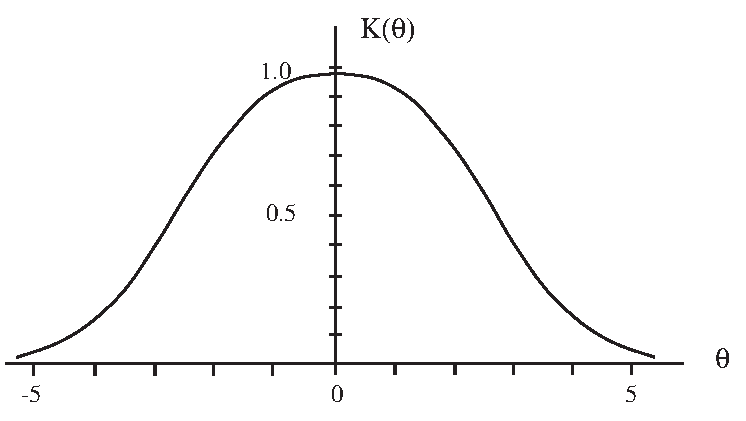
\includegraphics[scale=1.0]{figurer/fig15_3.pdf} 
\caption{Karakteristikk}
	\label{fig:karakteristikk2}
\end{figure}

\begin{figure}[ht]
\centering
	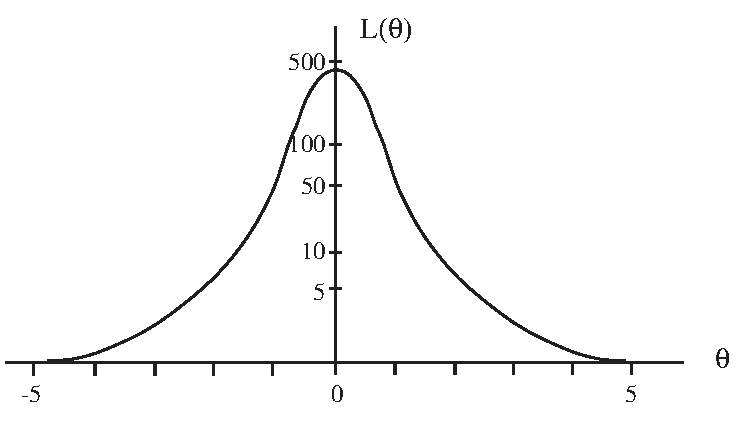
\includegraphics[scale=1.0]{figurer/fig15_4.pdf} 
\caption{Forventet tid til alarm}
	\label{fig:alarm}
\end{figure}

For den kontrollplanen vi her studerer vil bruk av $K(\theta)$ og
$L(\theta)$ være ekvivalent, men i praksis mener mange at bruk av
$L(\theta)$ er mer meningsfylt, fordi den sier noe om hvor mye av en
gitt kvalitet som blir akseptert i gjennomsnitt før alarm inntreffer.
Funksjonen $L(\theta)$ kan se ut som på Figur~\ref{fig:alarm}, merk at det har 
vært nødvendig å bruke logaritmisk skala på den vertikale
aksen for at figuren ikke skal forsvinne ``i det blå".


\noindent Vi har tidligere antydet at man også kunne gjøre bruk av 
varselgrensene.  La oss se på følgende kontrollplan:

\begin{quote}
    Alarm dersom et punkt faller utenfor alarmgrensene, eller to 
    suksessive punkter faller mellom varsel- og alarmgrensen på
    samme side.    
\end{quote}

\noindent Det kan vises at forventet antall kontroller inntil alarm som
 funksjon av $\theta$ nå blir

\[  L(\theta )=\frac{1+K_1(\theta )}{1-K_0(\theta )-K_0(\theta )\cdot K_1(\theta )}  \]

\noindent der $K_0(\theta )$ er sannsynligheten for at et punkt faller mellom 
varselgrensene, og $K_1(\theta )$ er sannsynligheten for at et punkt faller 
mellom en varsel- og den tilhørende alarmgrense.  Vi ser at $K_0(\theta)$
finnes på samme måte som $K(\theta)$ ved å bruke formelen med
$k_V$ istedenfor $k_A$, mens $K_1(\theta) = K(\theta) - K_0(\theta)$.

Den planen som her er foreslått kan sammenlignes med den enklere
planen ovenfor ved å studere $L(\theta)$ funksjonen for de to
planene.  Det ser ut til at den siste planen, med fornuftig valg av
$k_A$ og $k_V$, vil være å foretrekke framfor den første.  
For samme forventede ventetid til falsk alarm når prosessen er i 
kontroll, vil den siste planen gjennomgående være raskere til 
å oppdage reelle endringer.

I praksis ser en ofte valgt $k_A$ = 3 og $k_V$ = 2.  For en prosess som
er i kontroll, vil dette svare til at sannsynligheten ${\Pi}_A$ for et
punkt utenfor alarm\-grensene er ca. 0.0026, mens sannsynligheten
${\Pi}_V$ for et punkt utenfor varselgrensene er ca. 0.0456.  Noen
bruker isteden $k_A$ = 3.09 og $k_V$ = 1.96 svarende til 
sannsynlighetene 0.002 og 0.05.  Hva antall observasjoner $n$ ved hver
kontroll angår, brukes gjerne $n$ i området fra 4 til 10, som
oftest $n$ = 4 eller 5, altså et relativt lite antall observasjoner
ved hver kontroll.  Dette skyldes bl.a. at for å oppdage reelle 
endringer raskt, vil det erfaringsmessig være bedre å ta et lite
antall observasjoner relativt ofte enn et større antall noe sjeldnere,
mens det siste på den annen side vil være billigere.\\

\begin{eksempel}{Prosesskontroll}
Anta at vi bruker et kontrollsystem med alarm og varselgrenser gitt ved
$k_A = \pm 3$ og $k_V = \pm 2$.  Anta at ${\mu}_0$ = 10.0, 
$\sigma$ = 1.0 og $n$ = 4.  Vi er spesielt interessert i at endringer 
av forventet kvalitet $\mu$ til 11.5 eller mer skal oppdages raskt, dette
svarer til

\[  \theta =\frac{\mu - {\mu}_0}{\sigma /\sqrt{n}}=3 \]

\noindent Ved bruk av formlene ovenfor og Tabell~\ref{tab:Normal_Kurvenareal} og ~\ref{tab:Normal_Kurvefraktiler} i Appendiks~\ref{app:fordelngstabeller}, får vi 
følgende resultater (sjekk!)

\begin{center}
\begin{tabular}{|c|ccccc|} \hline
$\theta$       &      0     &     1     &     2     &     3     &   4 \\ \hline
$K(\theta)$    &   0.9974   &  0.9772   &  0.8413   &  0.5000   &  0.1587 \\
$K_0(\theta )$ &   0.9544   &  0.8400   &  0.5000   &  0.1587   &  0.0228 \\
$K_1(\theta )$ &   0.0430   &  0.1372   &  0.3413   &  0.3413   &  0.1359 \\
$L(\theta )$   &     229    &    25     &  4.0      &  1.7    &  1.2 \\ \hline
\end{tabular}
\end{center}

\noindent Vi ønsker å sammenligne denne plan med en plan uten varselgrenser
med omlag samme $L(0)$, dvs. samme forventet ventetid til første falske
alarm.  Dette betyr at siden $L(0) = 1/(1 - K(0))$, må $K(0)$ for
denne plan være

\[  K(0)=(L(0)-1)/L(0)=(229-1)/229=0.9956       \]

\noindent Dette svarer til $k_A$ = 2.85, dvs. som ventet noe mindre $k_A$ enn
for planen hvor alarm også kan inntreffe med to suksessive varsler.
Med $k_A$ = 2.85 får vi

\begin{center}
\begin{tabular}{|l|ccccc|} \hline
$\theta$     &     0     &     1     &     2     &     3     &     4 \\ \hline
$K(\theta )$ &  0.9956   &  0.9678   &  0.8023   &  0.4404   &  0.1251 \\
$L(\theta )$ &    229    &    31     &  5.1      &  1.8      &  1.1 \\ \hline
\end{tabular}
\end{center}
Vi ser at begge planer gjør jobben med å oppdage $\theta$ = 3
relativt raskt, mens planen med varselgrenser ser ut til å oppdage
små endringer noe raskere. \\
\end{eksempel}

Merk at sannsynlighetsbetraktningene ovenfor er knyttet til uavhengighet og
normaltilnærming (sentralgrensesetningen). Det kreves ikke absolutt at
observasjonene selv er normalfordelte. Unntatt er selvfølgelig når n er
liten, herunder spesielt $n=1$.


De kontrollplaner som er beskrevet til nå tar sikte på å
avdekke evt. endring i kvalitetsnivå $\mu$, mulige endringer
i variansen ${\sigma}^2$ er holdt utenfor.  Den teori som er utviklet
forutsetter at variansen fortsatt er den samme selv etter at prosessen
er løpt ut av kontroll.  Man kan imidlertid studere egenskapene ved 
disse kontrollplanene dersom vi også tillater at prosessen løper
ut av kontroll ved at variansen endres, i praksis vil den som regel
alltid øke.  Rent intuitivt er det vel klart at sjansen for alarm 
øker når variansen øker, men i hvilken grad krever teoretisk
analyse.

I mange situasjoner vil eventuelle endringer i variansen være like
viktig som endringer i nivået, ja endog være av primær
interesse.  Det er derfor utviklet egne kontrollplaner som tar sikte
på å føre kontroll med spredningen av observasjonene.  Vi
vil komme tilbake til dette nedenfor.

Anta at kontrollproblemet isteden dreier seg om en løpende 
produk\-sjons\-prosess hvor artiklene kun blir klassifisert som intakte 
eller defekte.  For kontrollformål undersøkes regelmessig $n$
artikler av produksjonen og antall defekte noteres.  Dette gjentas
etter gitte tidsintervaller.  Den teori vi har utviklet ovenfor gjelder 
i grove trekk også for denne situasjonen dersom vi plotter

\[   Z=\frac{X-np_0}{\sqrt{np_0(1-p_0)}}      \]

\noindent der $p_0$ er den defektsannsynlighet som svarer til at prosessen er 
i kontroll.  Merk at eventuelle reduksjoner i defektsannsynligheten
neppe vil ha alvorlige konsekvenser, men det vil også ha interesse
å finne ut om noe slikt har skjedd, og man bruker derfor vanligvis
alarmgrenser på begge sider av kontrollnivået likevel.  Merk
at for små $n$ og $p_0$ vil det ikke være rimelig å bruke
normaltilnærming ved beregning av alarmsannsynligheter, disse 
bør tas direkte ut fra en binomisk tabell.  I slike situasjoner vil
det også være aktuelt å plotte antall defekte istedenfor
den standardiserte størrelsen.

Den metode for prosesskontroll som er beskrevet ovenfor kalles i 
litteraturen ofte for {\em Shewharts metode}.  Det finnes andre metoder
som bygger på helt andre prinsipper.  Mest aktuell er kanskje den
såkalte {\em kumulativ-sum metoden:}

La $X_i$ for $i = 1, 2, 3, \ldots$ være observerte kvaliteter på
etterfølgende tids\-punkter for en produksjonsprosess.  Når 
prosessen er i kontroll oppfattes disse som uavhengige observasjoner
med forventning ${\mu}_0$.  Betrakt den kumulative sum

\[     Y_t=\sum_{i=1}^t(X_i-{\mu}_0)         \]

\noindent Dersom kvalitetsnivået for produksjonen er $\mu$ og ikke ${\mu}_0$
ser vi at 

\[ EY_t=(\mu-{\mu}_0)\cdot t        \]

\noindent Dette motiverer at vi kan holde prosessen under oppsikt mht. 
kvalitets\-nivå ved å plotte $Y_t$ som funksjon av $t$ ettersom 
observasjonene foreligger.  Så lenge prosessen er i kontroll, dvs.
$\mu = {\mu}_0$, vil $Y_t$ variere omkring null, men dersom prosessen
er ute av kontroll, slik at kvalitets\-nivået isteden er 
${\mu}_1 \neq {\mu}_0$, vil $Y_t$ variere omkring en linje med 
vinkelkoeffisient ${\mu}_1 - {\mu}_0$.  Dette indikerer at så snart
$Y_t$-plottet viser en systematisk trend forskjellig fra den 
horisontale linje så gir det grunn til å tro at noe er skjedd
mht. kvalitetsnivået i produksjonsprosessen.  Vi vil ikke her gå
i detalj med hvordan alarmgrenser konstrueres, men må vise til
spesiallitteratur.

En sammenligning av Shewharts metode og kumulativ-sum metoden viser
at små endringer i kvalitetsnivået har større sjanse for
å bli oppdaget raskere ved kumulativ-sum metoden enn ved Shewharts 
metode, det vil riktignok kunne ta en viss tid med begge metoder.  På
den annen side vil en betydelig endring i kvalitetsnivå ha størst
sjanse for å bli oppdaget raskt ved Shewharts metode, da det alltid 
tar noe tid før en stigende eller fallende trend blir åpenbar
ved plotting av den kumulative sum.

La oss til slutt kort se på hvordan vi kan føre kontroll med 
spredningen av kvalitet i produksjonsprosessen:  Anta at variansen,
når prosessen er i kontroll, er gitt lik ${\sigma}_0^2$.  La oss
tenke oss at prosessen kan gå ut av kontroll ved at variansen 
øker, la oss si til en ny verdi ${\sigma}^2 > {\sigma}_0^2$, en 
reduksjon er i praksis lite aktuelt.  Igjen tenker vi oss at etter visse
tidsintervaller observerer $n$ artikler av produksjonen som 
kvalitetsvurderes.  Som mål for spredningen av kvaliteten kan vi
beregne

\[  S^2=\frac{1}{n-1}\sum_{i=1}^{n}{(X_i-\bar{X})}^2 \]

\noindent Vi vet at $ES^2 = {\sigma}^2$, slik at dersom en observert $S^2$ er
stor i forhold til ${\sigma}_0^2$, gir dette grunn til å tro at
 ${\sigma}^2$ er større enn ${\sigma}_0^2$.  Som kontrollstørrelse 
velger vi å bruke

\[   W=S^2/{\sigma}_0^2     \]

\noindent som kan plottes i et kontrollskjema etter hvert som nye
stikkprøver av produksjonen foretas.  Vi velger å aksjonere
straks $W$ har verdi større enn $k$.  Sannsynligheten for ikke-aksjon,
også her kalt karakteristikken, vil vi betrakte som funksjon av
$\theta = {\sigma}/{\sigma}_0$ dvs. forholdet mellom det virkelige
standardavvik og det ``normale".  Vi har altså

\[   K(\theta )=P_{\theta}(W\leq k)   \]

\noindent For å kunne gi en spesifikk beregningsformel trenger vi derfor
å kjenne sannsynlighetsfordelingen til $W$.  Dersom vi er villige til å
anta at $X$-observasjonene oppfyller kravene i målemodellen og er
normalfordelte, kan det vises at fordelingen til

\[  Q=\frac{1}{\sigma^2}\sum_{i=1}^n{(X_i-\bar{X})}^2 \]

\noindent er eksakt lik kjikvadratkurven med $n-1$ frihetsgrader (se Kapittel
7.7).  Vi merker oss at $W\leq k$ er ekvivalent med at 
$Q\leq (n-1)\cdot k/{\theta}^2$ slik at karakteristikken blir
\begin{eqnarray*}
K(\theta )&=&P_{\theta}(Q\leq (n-1)\cdot k/{\theta}^2)\\
          &=&F_{n-1}((n-1)\cdot k/{\theta}^2)
\end{eqnarray*}

\noindent der $F_{n-1}(y)$ betegner arealet til venstre for $y$ under 
kjikvadratkurven med $n-1$ frihetsgrader.  Vi ser at karakteristikken,
for gitt $n$ og $k$, som ventet er avtagende i $\theta$.  Selv om
formelen ovenfor er utledet under normalitetsforutsetninger, vil
de tall som regnes ut også generelt gi en viss innsikt i egenskapene
ved ulike planer.

Den metode for spredningskontroll som er beskrevet her virker uansett
om prosessen løper på det opprinnelige kvalitetsnivå eller
har tilpasset seg et nytt nivå.  I praksis vil en derfor som regel
trenge å føre kontroll med både nivåendringer og
spredningsendringer. \\

\begin{eksempel}{Spredningskontroll}
Anta at $n$ = 4.  La oss prøve to ulike valg av alarmgrense, nemlig
$k$ = 2 og 3.  Ved hjelp av Tabell~\ref{tab:Kjikvadrat_Areal} har vi funnet følgende:

\begin{center}
\begin{tabular}{|c|cccccccc|} \hline
   & $\theta$ &  1.0  &  1.2  &  1.5  &  2.0  &  2.5  &  3.0  &  4.0 \\ \hline
$k$=2&$K(\theta )$ & 0.89 & 0.75 & 0.56 & 0.32 & 0.19 & 0.12 & 0.04 \\
$k$=3&$K(\theta )$ & 0.97 & 0.90 & 0.73 & 0.48 & 0.30 & 0.20 & 0.10 \\ \hline
\end{tabular}
\end{center}
Tabellen viser at den første planen har 11\% sjanse for falsk 
alarm ved en kontroll, den andre bare 3\%.  På den annen side vil
sjansen for å oppdage en dobling av standardavviket $(\theta = 2)$
være henholdsvis 68\% og 52\% for de to planene.\\
\end{eksempel}

Som i tilfellet med kontroll av kvalitetsnivå kan vi studere 
planer med både alarm og varselgrenser, eventuelt både øvre
og nedre slike.  Vi kan også betrakte forventet ventetid til
alarm etter de samme retningslinjer som ovenfor.  Litteraturen beskriver
også planer for spredningskontroll som istedenfor
empiriske varianser, tar utgangspunkt i variasjonsbredden dvs.
differensen mellom største og minste verdi av de $n$ $X$-observasjonene.\\

I praksis finnes mange typer kontrolldiagram og ulike tillempninger av slike.
Vi har her begrenset oss til å belyse koblingen til
sannsynlighetsregning og statistisk teori.\\[0.2cm]

\noindent {\bf Merknad.} Dersom man har grunn til å anta at en prosess
er i kontroll, er det verdiløst å foreta inspeksjon av et ferdig
parti som i avsnitt 15.2, med sikte på aksept eller forkastning av partiet,
se Oppgave~18. Dette er et sterkt argument for at kvalitetsarbeid må
rettes mot selve produksjonsprosessen.

\section{Kvalitetsforbedring}
Det beste utgangspunkt for forbedring av en prosess vil være når
prosessen er i kontroll.
Et kontrolldiagram som beskrevet i forrige avsnitt kan da tjene som et
``lytte"- og diagnoseverktøy, der påfallende mønstre i
observasjonene muligens kan tilskrives en spesiell årsak.

Det første trinn i kvalitetsforbedring av en prosess, vil være å
identifisere slike årsaker, og deretter fjerne dem, slik at vi sitter
igjen med en prosess i kontroll.
En slik prosess varierer tilfeldig rundt et nivå med konstant 
avvikstendens.  Denne variasjon har sjelden noen enkelt årsak,
men er typisk forårsaket av mange små årsaker som lite kan 
gjøres noe med, uten å endre prosessen på en mer fundamental
måte.  Det vil faktisk virke mot sin hensikt å reagere på 
enkeltavvik fra nivået som er innenfor grensene for tilfeldige avvik.\\

\noindent {\bf Merknad.} Grensene som prosessen i kontroll naturlig varierer mellom,
kalles vanligvis {\em kontrollgrenser}. Slike grenser må begrepsmessig ikke
forveksles med aksjonsgrenser som presentert i forrige avsnitt, ei
heller med spesifikasjonsgrenser, slike som ofte uttrykkes i 
bransjestandarder.\\

Vanligvis vil nivå $\pm$ $3\times$ standardavvik kunne fungere som
kontrollgrenser.
Med en prosess i kontroll har vi to muligheter mht. å bedre 
kvaliteten: endre kvalitetsnivået og redusere variasjonen.  Det vil
som regel være en rekke faktorer som er bestemmende for kvalitet,
så som produktdesign, maskindesign, produksjonsrutiner og
råmaterialer.

Statistisk eksperimentplanlegging og analyse kan bidra til å finne
bedre kombinasjoner av faktorer enn de som er i bruk til nå.  Det er
ofte mulig å gruppere faktorer i henhold til om de i hovedsak kan
påvirke nivå eller varia\-sjon, og det kan være et 
spørsmål hvilke en bør gripe fatt i først, eller om de kan 
studeres samtidig.  I denne forbindelse kan bruk av  målfunksjoner
som kombinerer de to karakteristika ved prosessen være aktuelle.
Mange foretrekker å angripe variabilitet først, og når denne
er redusert studeres mulighet for forbedring i nivå.  La oss fokusere
på forbedring i nivå.  Det er ofte mange faktorer som kan 
påvirke kvalitetsnivået.  Dersom hver faktor ønskes
studert på flere enn to nivåer, blir det i alt mange mulige 
faktorkombinasjoner, og med flere observasjoner pr. faktorkombinasjon,
vil omfanget av eksperimentet bryte grenser for det som er praktisk og
økonomisk forsvarlig å gjennomføre.  En må da forsøke 
å inngå kompromisser mht. eksperimentplan, f.eks. ved å
\begin{itemize}
\item  begrense seg til faktorer som anses mest vesentlige,     
\item  redusere antall nivåer for hver faktor, f.eks. til 2,
\item  la være å observere enkelte faktorkombinasjoner, 
\item  begrense seg til (høyst) en observasjon pr. faktorkombinasjon.  
\end{itemize}
Ved alle disse forslag risikerer en å tape noe, og valg av 
eksperimentplan må skje med åpne øyne, slik at vesentlig
informasjon har minst mulig sjanse for å unnslippe.

Fjerning av faktorer uten nærmere undersøkelse kan medføre
at uventede kvalitetspåvirkende effekter forblir uoppdaget.  Ved 
reduksjon av antall nivåer til to, vil ikke-lineære effekter
ikke kunne oppdages (i første omgang).  Ved å la være å
observere enkelte faktorkombinasjoner risikerer en at enkelte effekter
ikke lar seg identifisere, med mindre en velger spesielle 
eksperimentplaner, og gjør tilleggsantakelser om effektene.  Ved å
observere hver faktorkombinasjon bare en gang, kan en vanskelig anslå
usikkerhet, med mindre en gjør bestemte antakelser om fravær av
mer kompliserte effekter (samspill).

Det har i praksis vist seg at en kan lære mye, selv når en 
begrenser seg til to nivåer (f.eks. Lav/Høy) for hver faktor.  Vi
skal nedenfor gi en smakebit på fremgangsmåten i slike situasjoner.

Vi tenker oss at hver faktor kan påvirke responsen direkte ved
såkalte hovedeffekter som adderes opp.  I tillegg kan det tenkes at
bestemte kombinasjoner av faktorer påvirker responsen ut over dette.
Vi kaller dette {\em samspillseffekter}, se Kapittel 11.4 for mer formell
diskusjon.
Her brukes en noe enklere notasjon, som i tilfellet med to nivåer for
hver faktor, lettere lar seg generalisere til mange faktorer.\\

\begin{eksempel}{Et $2^2$-eksperiment}
Ved overflatebehandlingen av et produkt brukes et kjemikalium som 
vurderes tilsatt i to ulike styrkegrader (Faktor A: Lav/Høy), 
ved to ulike temperaturer (Faktor B: Lav/Høy).
Kvaliteten av finishen måles (høyere tall jo bedre). Det er gjort 2
observasjoner for hver av de $2^2 = 4$ faktorkombinasjonene, og resultatet ble
\begin{center}
\begin{tabular}{|c|cc|c|cc|cc|} \hline
Faktor-     & \multicolumn{2}{c}{Faktor}& &\multicolumn{2}{c|}{Observasjoner}
               &\multicolumn{2}{c|}{Gjennomsnitt/}   \\
kombinasjon & A & B  & AB  & nr. 1  &  nr.2  & 
                                \multicolumn{2}{c|}{Standardavvik}\\ \hline
   1   &$-$&$-$ &  +  &  45    &   47   &  $\bar{X}_1$ = 46  &  $S_1$ = 1.4\\
   2   & + &$-$ & $-$ &  40    &   40   &  $\bar{X}_2$ = 40  &  $S_2$ = 0.0 \\
   3   &$-$& +  & $-$ &  53    &   49   &  $\bar{X}_3$ = 51  &  $S_3$ = 2.8\\
   4   & + & +  &  +  &  50    &   53   &  $\bar{X}_4$ = 52  &  $S_4$ = 1.4\\ \hline
\end{tabular}
\end{center}
Her er faktorkombinasjonene nummerert fortløpende og er beskrevet for
hver faktor med koder $-/+$ for Lav/Høy.  Ved å ``multiplisere"
kodene for $A$ og $B$ får vi en nyttig kode for samspillet $AB$.
Denne er $+$ når begge faktorer er på samme nivå, og $-$
når faktorene er på motsatt nivå.  Observasjonene og deres
gjennomsnitt og standardavvik er ført ut til høyre for hver 
faktorkombinasjon.

Estimatorer for ulike effekter blir:
\begin{eqnarray*}
\mbox{Hovedeffekt} A:&\frac{1}{2}((\bar{X}_2-\bar{X}_1)+(\bar{X}_4-\bar{X}_3))&=-2.5\\
\mbox{Hovedeffekt} B:&\frac{1}{2}((\bar{X}_3-\bar{X}_1)+(\bar{X}_4-\bar{X}_2))&=8.5\\
\mbox{Samspill\ \ }AB:&\frac{1}{2}((\bar{X}_4-\bar{X}_3)-(\bar{X}_2-\bar{X}_1))&=3.5
\end{eqnarray*}
Disse svarer til $+$ kategorien for hver faktor, og estimater for $-$
kategorien fås ved å skifte fortegn (summen er null).  Legg
merke til at alle beregninger har form

\[ \frac{1}{2}(\pm \bar{X}_1 \pm \bar{X}_2 \pm \bar{X}_3 \pm \bar{X}_4) \]
der fortegnene er gitt ved de respektive $-/+$ koder for hver effekt.

Begrunnelsen for formlene ovenfor kan skje ut fra formlene i 
Kapittel 11.4 eller direkte.  Estimatene for hovedeffekten $A$ får
vi ved å beregne gjennomsnittet av endringene fra Lav til Høy 
for $A$ for de to mulige nivåer for $B$, og ta gjennomsnittet av disse.
Tilsvarende for hovedeffekten $B$.  Samspillet $AB$ anslås ved å
se på forskjellen i anslått endring fra Lav til Høy, for $A$,
for henholdsvis Høy og Lav for $B$.

Anslagene ovenfor bør vurderes i lys av sine standardavvik.  Som
regel beregnes dette under antakelsen at uavhengige enkeltobservasjoner
med samme standardavvik $\sigma$ uansett faktorkombinasjon.  Da er 
variansen til estimatorene ovenfor ${\sigma}^2/m$, der $m$ er antall
gjentatte observasjoner for hver faktorkombinasjon (i eksemplet er
$m$ = 2).  Anslag for ${\sigma}^2$ blir da

\[       S^2=\frac{1}{4}(S_1^2+S_2^2+S_3^2+S_4^2) \]
der $S_i$ er beregnet standardavvik for observasjonene ved 
faktorkombinasjon  nr. $i$.
Estimator for standardavviket til effektestimatorene blir derfor
$S/\sqrt{m}$, og vi kan rapportere

\[    \mbox{Effektestimat} \pm \frac{S}{\sqrt{m}}       \]
med vanlig grov fortolkning av feilmarginer.  Ved antakelse om 
normalfordelte observasjoner kan en lage eksakte konfidensintervaller
der en putter inn en sikkerhetsfaktor etter oppslag i $t$-fordelingen
med $4(m-1)$ frihetsgrader.

I eksemplet ovenfor beregner vi $S$ = 1.72, som gir estimert
standardavvik lik 1.21.  Av resultatene ser vi en klar temperatureffekt
i favør av høy temperatur, og en ikke signifikant styrkeeffekt
i favør av lav kjemikaliestyrke.  Imidlertid ser vi en mulig
samspilleffekt

\[         3.5 \pm 1.21 .        \]
Et 95\% konfidensintervall vil med 4 frihetsgrader kreve 
sikkerhetsfaktor $k$= 2.776, som gir konfidensgrenser $3.5 \pm 3.36$.
Det kan altså se ut som at høy kjemikaliestyrke er gunstig
i kombinasjon med høyere temperatur.  En går da selvsagt inn for denne
 kombinasjonen, selv om hovedeffekten av $A$ favoriserer lav kjemikaliestyrke.
I praksis vil en helst ikke rapportere vha. hovedeffekter og samspill i 
situasjoner der samspill er mer enn en tredjedel av hovedeffekter.\\
\end{eksempel}

\begin{eksempel}{Et $2^3$-eksperiment}
Anta at vi i forrige eksempel kan tenkes å velge en av to 
dyseåpninger (Faktor C: Lav/Høy) i tillegg til faktorene $A$ og $B$.
Vi har da følgende skjema med resultater med to observasjoner pr.
faktorkombinasjon.
\begin{center} \addtolength{\tabcolsep}{-0.1\tabcolsep} 
\begin{tabular}{|l|ccc|ccc|c|cc|} \hline
Faktor-     & \multicolumn{3}{c|}{Faktorer}& \multicolumn{4}{c|}{Samspill} &
                                              Gj.snitt &  St.avvik   \\
kombinasjon &  A & B & C  &  AB & AC & BC &  ABC &$\bar{X}_i$& $S_i$\\ \hline
  1         & $-$&$-$&$-$ &  +  & +  & +  &  $-$ &    49     &  1.0    \\  
  2$\star$  &  + &$-$&$-$ & $-$ &$-$ & +  &   +  &    43     &  1.7  \\
  3$\star$  & $-$& + &$-$ & $-$ & +  &$-$ &   +  &    52     &  1.7  \\
  4         &  + & + &$-$ &  +  &$-$ &$-$ &  $-$ &    54     &  2.4 \\
  5$\star$  & $-$&$-$& +  &  +  &$-$ &$-$ &   +  &    46     &  1.4 \\
  6         &  + &$-$& +  & $-$ & +  &$-$ &  $-$ &    40     &  0.0  \\
  7         & $-$& + & +  & $-$ &$-$ & +  &  $-$ &    51     &  2.8 \\
  8$\star$  &  + & + & +  &  +  & +  & +  &   +  &    52     &  1.4 \\ \hline
\end{tabular}
\end{center}
Her vil alle estimatorer for hovedeffekter og samspill ha form

\[ \frac{1}{2^{3-1}}(\pm \bar{X}_1\pm \bar{X}_2\pm \ldots \pm \bar{X}_8) \]
der $-/+$ velges i henhold til skjemaet ovenfor.  Standardavvikene til
estimatoren kan estimeres med $S/\sqrt{2m}$ (begrunnes som ovenfor),
der $m$ er antall observasjoner pr. faktorkombinasjon og 

\[       S^2=\frac{1}{8}(S_1^2+S_2^2+ \ldots +S_8^2) \]
Dersom vi antar normalfordelte observasjoner, kan sikkerhetsfaktorer 
beregnes ut fra $t$-fordelingen med $8(m-1)$ frihetsgrader. 
Hovedeffekter og samspill blir anslått til:
\begin{center}
\begin{tabular}{ccccccc}
 $A$ & $B$ & $C$ & $AB$ & $AC$ & $BC$ & $ABC$ \\
 -2.25& 7.75&-2.25& 3.75 &-0.25 &-0.75 &-0.25
\end{tabular}
\end{center}
Her blir $S$=1.77, som gir estimert standardavvik lik 0.88.
Det ser ut til at $C$ ikke er involvert i samspill, men at $C$ har signifikant
 hovedeffekt i favør av lav dyseåpning.
\end{eksempel}

Man har ofte ikke anledning til flere enn en observasjon pr. faktorkombinasjon.
Det er da ikke mulig å anslå $S$ som ovenfor, men det fins
måter for mer uformell betraktning av usikkerheten.

Med bare to nivåer for hver faktor vil en, selv med et moderat antall
faktorer, få mange kombinasjoner. Eksempelvis gir 8 faktorer
$2^8$ = 256 kombinasjoner.  I praksis er det ofte bare et fåtall 
faktorer som påvirker responsen ofte 2 - 3 (Paretoprinsippet).
Det fins eksperimentplaner, såkalte {\em fraksjonerte planer}, der en ikke
observerer alle faktorkombinasjoner, men er likevel i stand til å
avdekke alle samspill mellom to faktorer, men ikke nødvendigvis
mer kompliserte samspill, som likevel sjelden forekommer i praksis.
I eksemplet ovenfor er det f.eks. nok å observere faktorkombinasjonene
merket med $\star$, dersom vi antar at samspill mellom alle tre faktorene
ikke forekommer.

Det kan være vanskelig å få anledning til å 
gjennomføre eksperimenter i stor skala med prosesser som er i drift. 
Det er derfor utviklet eksperi\-mentplaner og statistiske metoder for
situasjoner der en trinnvis foretar små endringer som ikke medfører
driftsstans, som på noe sikt kan lede til optimal faktorkombinasjon,
såkalt ``Evolutionary Operations".

\section{Oppgaver}
\small
\begin{enumerate}
\item
Studer karakteristikken til følgende alternative planer for
situasjonen i Eksempel 1:
 (a) $n$ = 4 og $k$ = 0.2 \ \ \ (b) $n$ = 3 og $k$ = 0.1 \\
Kommenter resultatene.
\item
Finn produsentens og konsumentens risiko for planene i Oppgave~1 dersom
${\theta}_1 = 1/8$ og ${\theta}_2 = 4/8$.
\item
Finn forventet utgående kvalitet for hver av planene i Oppgave~1 dersom 
 \begin{itemize}
 \item[(a)] aksepterte partier sendes som de er, mens et forkastet parti 
    erstattes med et intakt.
 \item[(b)] alle funne defekte artikler i akseptert parti erstattes med intakte,
    mens et forkastet parti erstattes med et intakt.
 \item[(c)] aksepterte partier sendes som de er, mens forkastede partier ikke
    videresendes.
 \end{itemize}Finn også maksimum forventet andel defekte ved hver plan.
\item
Betrakt en kontrollplan der forkastning medfører at alle resterende
artikler i partiet også kontrolleres.  Finn forventet antall artikler
som må kontrolleres i alt som funksjon av $M$ dersom $N$ = 8 og
(jfr. Oppgave~1),\\
(a) $n$ = 4 og $k$ = 0, 1, 2 \ \ \ (b) $n$ = 3 og $k$ = 0, 1
\item
 (a) Bestem karakteristikkene og tegn disse i en figur for følgende planer
\begin{center}
\begin{tabular}{rclccc}
      (i) & $N$ = 2000 & $n$ = 100 & og & $k$ = 4 \\
     (ii) & $N$ = 2000 & $n$ = 50  & og & $k$ = 2 \\
    (iii) & $N$ = 2000 & $n$ = 25  & og & $k$ = 1 
\end{tabular}
\end{center}
 (b)Bestem produsentens og konsumentens risiko for
    ${\theta}_1$= 0.05   ${\theta}_2$= 0.10 \\
 (c) Bestem forventet utgående kvalitet for planene i (a) dersom aksepterte
\indent partier sendes som de er og hvert forkastet parti erstattes
med et intakt.
\item
Bestem en plan der produsentens risiko $\alpha$ og konsumentens risiko
$\beta$ er gitt ved $\alpha$ = $\beta$ = 0.05, beregnet for henholdsvis
${\theta}_1$ = 0.01 og ${\theta}_2$ = 0.05, i tilfellene 
(i) $N$ = 10 000  \ \ \     (ii)  $N$ = 1 000  \ \ \   (iii)  $N$ = 100
\item
En revisor har et større antall bilag av en viss type, og det er 
uaktuelt å gjennomgå alle disse med mindre en stikkprøve
skulle avsløre betydelige uregelmessigheter. \\
(a) Formuler situasjonen som et kvalitetskontrollproblem. \\
(b) Finn tilnærmet karakteristikken for følgende planer \\
 (i) $n$=40, $k$=0,\ \ (ii) $n$ = 80, $k$ = 1, \ \ (iii) $n$ = 100, $k$ = 1.\\
Er det nødvendig å kjenne $N$ eksakt for å besvare (b)?
\item
En produsent leverer partier av en vare bestående av $N$ = 25
enheter.  Disse kan variere noe i kvalitet og kan sorteres i to kvaliteter.
Det er ikke ønskelig at et levert parti inneholder mer enn to enheter
av annen sortering.  Mottakeren vurderer to ulike stikkprøvemetoder: 
\begin{itemize}
\item[(a)] Det trekkes 8 artikler og partiet aksepteres dersom antall defekte
    er høyst en.
\item[(b)] Trekk først 5 artikler. Dersom utvalget er uten defekte, 
   aksepteres partiet, mens dersom det er mer enn en defekt forkastes partiet.
    Ved akkurat en defekt trekkes nye 5 artikler og partiet aksepteres dersom
    dette utvalget er uten defekte, i motsatt fall forkastes det.
\end{itemize}
Sammenlign karakteristikken til de to metodene når enheter av annen 
sortering spiller rollen som defekte.
\item
Sammenlign begrepene i teorien for kontroll av produserte artikler med 
begrepene i hypotesetestingsteorien.  Drøft eventuelle sammenhenger
mellom \\
(a) Karakteristikk og styrkefunksjon. \\
(b) Konsumentens risiko og signifikansnivå. \\
(c) Produsentens risiko og styrke. \\
\item
En bestemt type snøre vil ved vanlige produksjonsforhold 
gjennom\-snitt\-lig tåle en belastning i kilo på 10.0, og man har 
erfaring for at standardavviket kan settes til 0.4.  Hver time velges
ut 4 snører som belastes.  Gjennomsnittlig belastning som tåles 
blir beregnet og danner utgangspunkt for føring av kontrolldiagram.
Anta først at kontrolldiagrammet har alarmgrensene $k_A = \pm 3$. 
\begin{itemize}
\item[(a)] Finn forventet ventetid til falsk alarm. 
\item[(b)] Finn forventet ventetid til alarm dersom kvalitetsnivået er
    endres til 9.5 kg og til 9.0 kg.
\end{itemize}
Anta at vi i tillegg bruker varselgrensen $k_V = \pm 2$.  Besvar (a) og
(b) dersom to etterfølgende varsler gir alarm.
\item
Følgende observasjoner på 8 etterfølgende tidspunkter 
foreligger for situa\-sjonen i forrige oppgave.
\begin{center}
\begin{tabular}{|r|rrrrrrrr|} \hline
Tidspunkt &  1   &   2   &   3   &   4   &   5   &   6   &   7  &   8 \\ \hline
Obs. nr.1 &  9.5 & 10.8  & 10.2  & 10.4  & 10.3  &  9.7  &  9.3 &  9.8 \\
        2 & 10.4 & 10.5  &  9.1  &  9.6  &  9.4  &  9.1  &  9.0 &  9.2 \\
        3 & 10.7 &  9.6  &  9.5  & 10.0  &  9.7  &  9.4  &  9.6 & 10.1 \\
        4 &  9.8 & 10.3  & 10.4  & 10.6  &  9.1  & 10.1  &  9.9 &  9.5 \\ \hline
\end{tabular}
\end{center}
\begin{itemize}
\item[(a)] Beregn standardiserte gjennomsnitt og plott disse i et 
kontrolldiagram med alarmgrenser $k_A = \pm 3$ og varselgrenser $k_V = \pm 2$.
\item[(b)] Gir tallmaterialet grunn til å aksjonere, i så fall når?
\end{itemize}
\item
En produksjonsprosess gir under vanlige omstendigheter 5\% defekte.  
Fra den løpende produksjon velges hver halvtime $n$ = 100 artikler
som testes og antall defekte noteres.  En dag var resultatet som følger:
\begin{center}
\begin{tabular}{l|rrrrrrrrrrrr}
Tidspunkt    & 1 & 2 & 3 & 4 & 5 & 6 & 7 & 8 & 9 & 10 & 11 & 12 \\ \hline
Defekte      & 3 & 7 & 5 & 1 & 7 & 4 & 9 & 7 & 9 &  6 & 10 &  9
\end{tabular}
\end{center}
\begin{itemize}
\item[(a)] Plott resultatene i et kontrolldiagram med alarmgrenser
 $k_A = \pm 3$ og varselgrenser $k_V = \pm 2$. 
\item[(b)] Gir tallmaterialet grunn til å aksjonere, i så fall når? 
\item[(c)] Hva er forventet ventetid til alarm fra et tidspunkt da prosessen 
    be\-gyn\-ner å gi gjennomgående 10\% defekte.
\end{itemize}
\item
I en situasjon med kontroll av defektprosenten i en produksjonsprosess
som under normale omstendigheter gir 10\% defekte velges $n$ = 10
artikler ut for testing hver halvtime.  Man ønsker å plotte antall
defekte artikler direkte i et kontrolldiagram med bare en øvre alarmlinje.
Bestem denne alarmlinjen i følgende situasjoner \\
(a) Forventet ventetid til falsk alarm skal være ca. 75. \\
(b) Forventet ventetid til alarm ved dobling av defektprosenten blir
     ca. 3. \\
Hvordan kan man eventuelt få oppfylt begge ønskemål (a) og (b)?
\item 
Anta at vi bruker planen i Oppgave~13~(a) og at vi har observert
\begin{center}
\begin{tabular}{l|rrrrrrrrrrrr}
Tidspunkt    &   1 & 2 & 3 & 4 & 5 & 6 & 7 & 8 & 9 & 10 & 11 & 12 \\ \hline
Defekte      &   1 & 2 & 0 & 2 & 1 & 0 & 2 & 2 & 1 &  3 &  1 &  2
\end{tabular}
\end{center}
Gir tallmaterialet grunn til å aksjonere, i så fall når?
\item
En bedrift vil føre kontroll med spredningen av kvalitet etter 
metoden beskrevet i teksten.  Anta at $n$ = 5.
\begin{itemize}
\item[(a)] Tegn karakteristikken $K(\theta)$ for tilfellet $k$ = 3.
\item[(b)] Hvilken verdi må $k$ ha for at sannsynligheten for falsk alarm 
    ved en kontroll skal være ca. 0.01? 
\item[(c)] Hva er sannsynligheten for alarm dersom standardavviket er doblet?
\end{itemize}
\item
Bestem en plan for spredningskontroll av den typen som er beskrevet i
teksten der forventet ventetid til falsk alarm er 200, mens forventet
ventetid til alarm ved en dobling av standardavviket er 5.  Finn
forventet antall artikler som passerer før alarmen går dersom
standardavviket er doblet.
\item
Man ønsker å føre kontroll med både nivå og spredning
av kvaliteten i den løpende produksjon, og regelmessig velges ut 9
artikler som kvalitetsmåles.  Under normale forhold har kvaliteten
til en tilfeldig valgt artikkel forventning 40.0 og standardavvik 3.0.
Anta at observerte gjennomsnitt $\bar{X}$ og estimerte standardavvik 
$S$ plottes direkte i hvert sitt kontrolldiagram.  For begge 
kontrolldiagrammer ønsker en at forventet ventetid til falsk alarm
av typen forverring skal være ca. 100.  Fastlegg kontrollplaner i
henhold til dette. Følgende observasjoner foreligger:
\begin{center}
\begin{tabular}{cccccccccc}
 $\bar{X}$: &  41.7 & 38.5 & 39.2 & 40.6 & 40.9 & 39.3 & 38.7 & 40.4 & 42.1 \\
        &  40.1 & 39.2 & 37.7 & 40.5 & 38.4 & 38.6 & 37.9 & 38.5 &       \\
        &       &      &      &      &      &      &      &      &       \\ 
 $S$:      &   3.7 &  2.8 &  2.2 &  3.4 &  3.3 &  3.1 &  2.6 &  2.9 &  3.4  \\
        &   3.9 &  3.2 &  4.0 &  4.2 &  3.9 &  4.8 &  4.2 &  4.6 &
\end{tabular}
\end{center}
Blir det slått alarm i løpet av disse 17 tidspunktene, i så
fall når, og hva slags alarm?

\item Anta at vi har en prosess som produserer artikler med konstant
     defektsannsynlighet $p$, der vi har uavhengighet over tid (prosessen er i
     kontroll). $N$ etterfølgende artikler fra denne prosessen utgjør et
parti, hvor det er et ukjent antall defekte $M$. Fra partiet trekkes $n$ artikler,
     og antall defekte $Y$ blant disse noteres.\\
    Vis at antall gjenværende defekte i partiet $X=M-Y$ er uavhengig av $Y$.\\
    Drøft konsekvensene av dette for partiinspeksjon i praksis.
\item Gjennomfør beregningene av de størrelser som er oppgitt i Eksempel 8,
   og lag deretter konfidensintervaller for hovedeffekter og samspill.
\item En fruktdrikk leveres i pappemballasje, og en vurderer tre ulike faktorer
   ved produksjonen. Et eksperiment ble utført der smak ble vurdert på en 
   skala fra 1 til 9 av en dommer. Resultatet ble
   \begin{center}
   \begin{tabular}{ccccc}
    Vokslag (A) & Luftrom (B) & Tilsetning (C) &
                                 \multicolumn{2}{c}{Observasjoner} \\ \hline
       Tynt     & Intet      & Lav   &  6  &  8 \\
       Tynt     & Intet      & Høy&  8  &  7 \\
       Tynt     & Lite       & Lav   &  9  &  9 \\
       Tynt     & Lite       & Høy&  1  &  2 \\
       Tykt     & Intet      & Lav   &  6  &  7 \\
       Tykt     & Intet      & Høy&  6  &  8 \\
       Tykt     & Lite       & Lav   &  9  &  8 \\
       Tykt     & Lite       & Høy&  2  &  3 \\ \hline
   \end{tabular}
   \end{center}
   Anslå hovedeffekter og samspill, og vurder deres signifikans, med
   sikte på finne den beste eller gode kombinasjoner av faktorene.
\end{enumerate}
\normalsize
